
\section{Benchmarking CIQ}
\label{sec:ciq_empirical}

In this section we empirically measure the convergence and speedup of CIQ applied to several types of covariance matrices.
%We demonstrate that
%\begin{enumerate*}
  %\item CIQ requires few quadrature points and msMINRES iterations for convergence; and
  %\item CIQ is faster than Cholesky for large matrices.
%\end{enumerate*}

\paragraph{Convergence of CIQ.}
In \cref{fig:quad_error} we measure the relative error of computing $\bK^{1/2} \bb$ with CIQ on random matrices.
We vary
%
\begin{enumerate*}
  \item the number of quadrature points $Q$;
  \item the size of the matrix $N$; and
  \item the conditioning of the matrix.
\end{enumerate*}
%
The left and middle plots display results for matrices with spectra that decay as $\lambda_t = 1 / \sqrt{t}$, $\lambda_t = 1/t$, $\lambda_t = 1 / t^2$, and $\lambda_t = e^{-t}$.
The right plots display results for one-dimensional Mat\'ern and RBF kernel matrices (formed with random data), which have near-exponentially decaying spectra.
Consequentially, the $1 / \sqrt{t}$ and $1 / t$ matrices are relatively well-conditioned while the Mat\'ern/RBF kernels are relatively ill-conditioned.
Nevertheless, in all cases CIQ achieves $10^{-4}$ relative error with only $Q=8$ quadrature points, regardless of the size of the matrix.

\begin{figure}[t!]
	\centering
	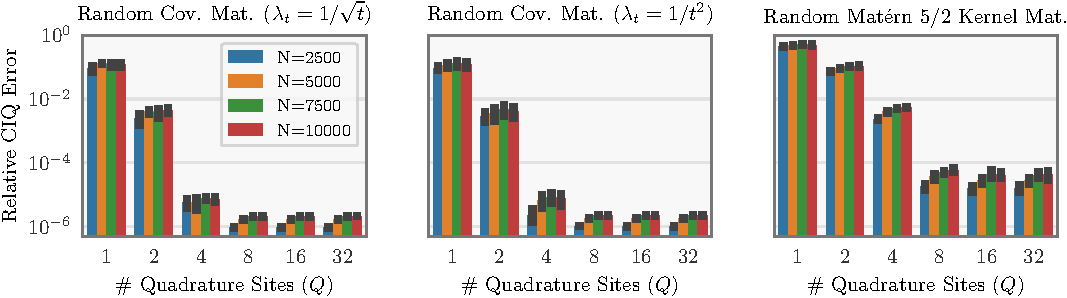
\includegraphics[width=\textwidth]{figures/quad_error.pdf}

	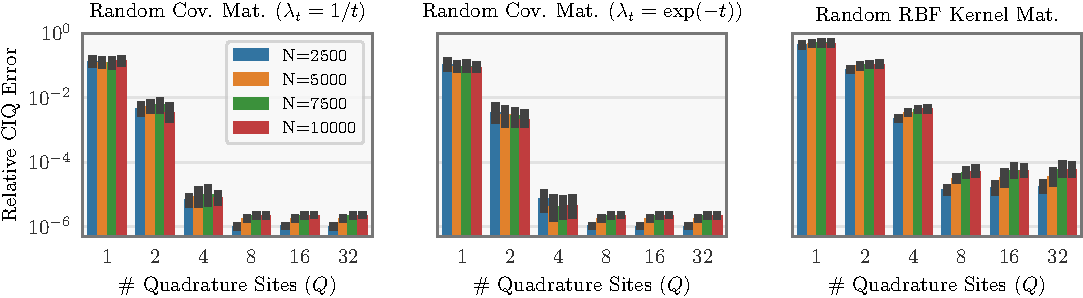
\includegraphics[width=\textwidth]{figures/quad_error_supp.pdf}
  \caption[
    Relative error of CIQ as a function of number of quadrature points $Q$.
  ]{
    CIQ relative error at computing $\bK^{1/2} \bb$ as a function of number of quadrature points $Q$.
    We test random matrices with eigenvalues that scale as $\lambda_t = 1/\sqrt{t}$ (top left), $\lambda_t = 1/t$ (bottom left), $\lambda_t = 1/{t}^2$ (top middle), and $\lambda_t = e^{-t}$ (bottom middle).
    Additionally, we test random Mat\'ern/RBF kernel matrices (top right/bottom right).
    In all cases $Q=8$ achieves $<10^{-4}$ error.
  }
  \label{fig:quad_error}
\end{figure}

Typically $J=100$ msMINRES iterations suffices for convergence; however this number can be lowered with preconditioning.
To demonstrate this, we construct  random $N \times N$ Mat\'ern/RBF kernels $\bK$, applying CIQ to a set of $N$ orthonormal vectors ($[\bK^{1/2} \bb_{1}, \ldots, \bK^{1/2} \bb_{N}]$), and compute the empirical covariance.
In \cref{fig:precond_result} we plot the number of msMINRES iterations needed to achieve a relative error of $10^{-6}$.
The pivoted Cholesky preconditioner of \cref{sec:preconditioning}---which forms a low-rank approximation of $\bK$---accelerates convergence of msMINRES.
Without preconditioning (i.e. rank=0), $J=100$ iterations are required for $N=7,\!500$ matrices.
With rank-100/rank-400 preconditioners, iterations are cut by a factor of two/four.

\begin{figure}[t!]
	\centering
	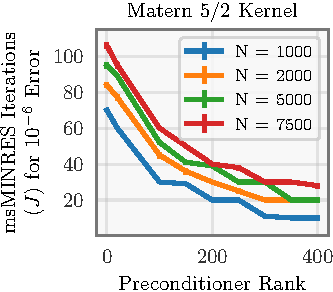
\includegraphics[width=0.4\textwidth]{figures/precond_result.pdf}
  \quad
	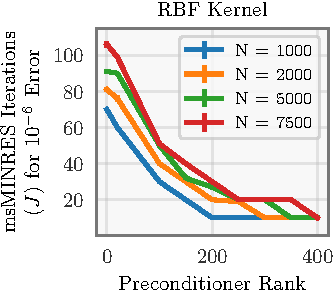
\includegraphics[width=0.4\textwidth]{figures/precond_result_rbf.pdf}
  \caption[
    Effect of preconditioning on CIQ convergence.
  ]{
    Effect of preconditioning on CIQ convergence (random Mat\'ern and RBF kernels with a pivoted Cholesky preconditioner \citep{gardner2018gpytorch}).
    Larger preconditioners reduce the number of msMINRES iterations required to reach $10^{-6}$ error.
  }
  \label{fig:precond_result}
\end{figure}

\begin{figure}[t!]
	\centering
	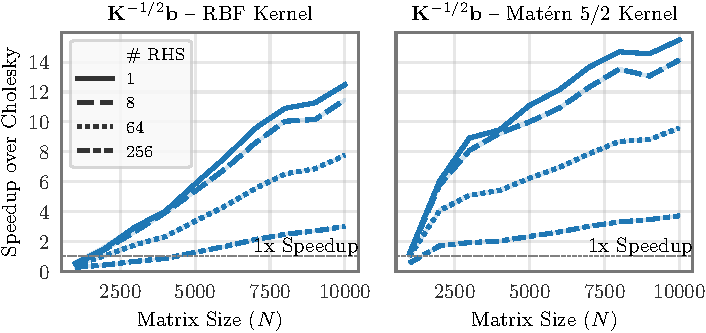
\includegraphics[width=0.8\textwidth]{figures/timing.pdf}
  \caption[
    Speedup of CIQ over Cholesky.
  ]{
    Speedup of CIQ over Cholesky when computing forward/backward passes of $\bK^{-1/2} \bb$ with varying number of right-hand-sides (RHS).
  }
  \label{fig:timing}
\end{figure}

\paragraph{Speedup over Cholesky.}
We compare the wall-clock speedup of CIQ over Cholesky in \cref{fig:timing} on RBF/Mat\'ern kernels.\footnote{
  $Q=8$.
  msMINRES is stopped after a residual of $10^{-4}$.
  Kernels are formed from the Kin40k dataset \citep{asuncion2007uci}.
  Timings are performed on a NVIDIA 1070 GPU.
}
We compute $\bK^{-1/2} \bb$ and its derivative on multiple right-hand-size (RHS) vectors.
As the $N$ increases, CIQ incurs a larger speedup (up to $15\times$ faster than Cholesky).
This speedup is less pronounced when computing many RHSs simultaneously, as the cubic complexity of Cholesky is amortized across each RHS.
Nevertheless, CIQ is computationally advantageous for matrices larger than $N=3,\!000$ even when simultaneously whitening $256$ vectors.
